\section{基本定义}

\subsection{左右手系}
\begin{frame}
\pause
(x,y,z)满足右手系的定义为伸出右手，将四指由x轴指向沿小于平角的叫转到y轴指向，拇指所指的方向为z轴方向。

左手系也可类似定义。

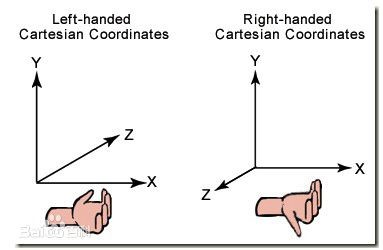
\includegraphics[height=3cm]{geometry/hand.png}

\end{frame}

\subsection{三维叉积}
\begin{frame}
\pause
三维叉积的计算是通过计算行列式$\left| \begin{array}{c @{\ } c @{\ } c} i & j & k \\ x_1 & y_1 & z_1 \\ x_2 & y_2 & z_2 \end{array} \right|$来得到的。

\pause
需要注意的是三维向量的叉积得到的还是一个向量$(y_1 z_2-y_2 z_1,x_2 z_1-x_1 z_2,x_1 y_2-x_2 y_1)$。

它的模长等于原来两个向量所围成的平行四边形的面积。
\end{frame}

\subsection{混合积}
\begin{frame}
\pause
$(\overrightarrow{a} \times \overrightarrow{b}) \cdot \overrightarrow{c}$ 为向量$\overrightarrow{a},\overrightarrow{b},\overrightarrow{c}$的混合积，它的含义是向量$\overrightarrow{a},\overrightarrow{b},\overrightarrow{c}$ 所围成的平行六面体的体积。
\end{frame}

\subsection{三维向量旋转}
\begin{frame}
\pause
三维空间中的旋转变换比二维空间中的旋转变换复杂。除了需要指定旋转角外，还需指定旋转轴。

若以坐标系的三个坐标轴x,y,z分别作为旋转轴，则点实际上只在垂直坐标轴的平面上作二维旋转。此时用二维旋转公式就可以直接推出三维旋转变换矩阵。

规定在右手坐标系中，物体旋转的正方向是右手螺旋方向，即从该轴正半轴向原点看是逆时针方向。
\end{frame}

\begin{frame}
\frametitle{绕坐标轴旋转}
\pause
\begin{multicols}{2}
Case \ 1:绕z轴旋转

$x'=x\cos(\gamma)-y\sin(\gamma)$

$y'=x\sin(\gamma)+y\cos(\gamma)$

$z'=z$

Case \ 2:绕x轴旋转

$y'=y\cos(\gamma)-z\sin(\gamma)$

$z'=y\sin(\gamma)+z\cos(\gamma)$

$x'=x$

Case \ 3:绕y轴旋转

$z'=z\cos(\gamma)-x\sin(\gamma)$

$x'=z\sin(\gamma)+\cos(\gamma)$

$y'=y$

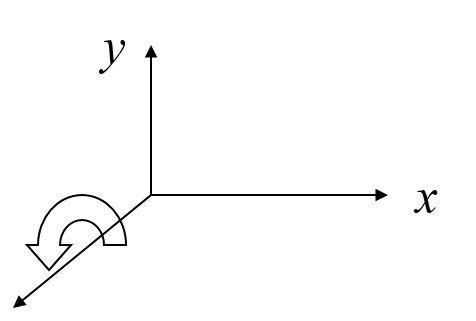
\includegraphics[height=2cm]{geometry/rotate1.png}

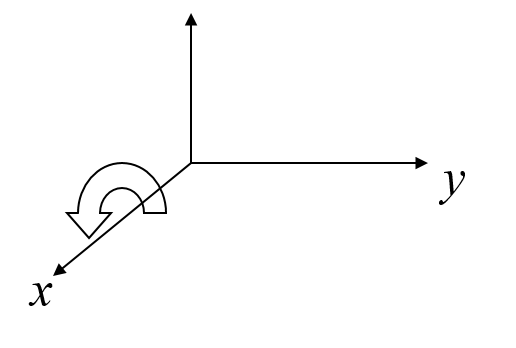
\includegraphics[height=2cm]{geometry/rotate2.png}

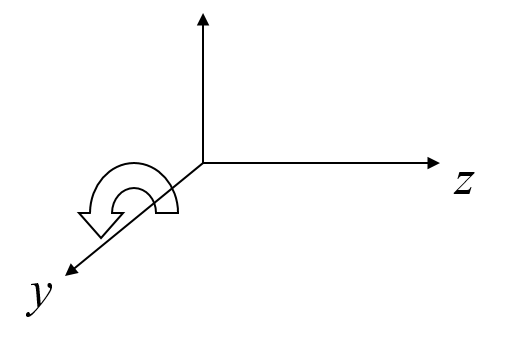
\includegraphics[height=2cm]{geometry/rotate3.png}
\end{multicols}
\end{frame}

\begin{frame}
\frametitle{绕坐标轴旋转}
\framesubtitle{旋转矩阵}
绕z轴:
$(x \ y \ z \ 1)
\left[
    \begin{array}{ c @{\ } c @{\ } c @{\ } c }
        \cos(\gamma)  & \sin(\gamma) & \ \ \ 0 \ \ \ & \ \ \ 0 \ \ \ \\
        -\sin(\gamma) & \cos(\gamma) & \ \ \ 0 \ \ \ & \ \ \ 0 \ \ \ \\
        0             & 0            & \ \ \ 1 \ \ \ & \ \ \ 0 \ \ \ \\
        0             & 0            & \ \ \ 0 \ \ \ & \ \ \ 1 \ \ \
    \end{array}
\right]
=(x' \ y' \ z' \ 1)$

绕x轴:
$(x \ y \ z \ 1)
\left[
    \begin{array}{ c @{\ } c @{\ } c @{\ } c }
       \ \ \ 1 \ \ \ & 0             & 0            & \ \ \ 0 \ \ \ \\
       \ \ \ 0 \ \ \ & \cos(\gamma)  & \sin(\gamma) & \ \ \ 0 \ \ \ \\
       \ \ \ 0 \ \ \ & -\sin(\gamma) & \cos(\gamma) & \ \ \ 0 \ \ \ \\
       \ \ \ 0 \ \ \ & 0             & 0            & \ \ \ 1 \ \ \
    \end{array}
\right]
=(x' \ y' \ z' \ 1)$

绕y轴:
$(x \ y \ z \ 1)
\left[
    \begin{array}{ c @{\ } c @{\ } c @{\ } c }
        \cos(\gamma)  & \ \ \ 0 \ \ \ & -\sin(\gamma) & \ \ \ 0 \ \ \ \\
        0             & \ \ \ 1 \ \ \ & 0             & \ \ \ 0 \ \ \ \\
        \sin(\gamma)  & \ \ \ 0 \ \ \ & \cos(\gamma)  & \ \ \ 0 \ \ \ \\
        0             & \ \ \ 0 \ \ \ & 0             & \ \ \ 1 \ \ \
    \end{array}
\right]
=(x' \ y' \ z' \ 1)$

\end{frame}

\begin{frame}
\frametitle{绕任意直线旋转}
\pause
有了绕坐标轴旋转的方法之后，就可以得到绕任意直线旋转的方法。\newline \newline

\pause
先把该向量变成以(0,0,0)为起点、(a,b,c)为终点，然后把该向量以x轴为旋转轴把向量旋入平面xy，再以y轴为旋转轴把向量旋入平面yz，这样最后的向量就变成了z轴，直接绕z轴旋转即可，旋转完毕之后再旋转回来。\newline \newline

\pause
分五次绕坐标轴旋转操作
\end{frame}

\begin{frame}
\frametitle{绕任意直线旋转}
\framesubtitle{第一步}
\pause
以x轴为旋转轴把向量旋入平面xy

旋转的角度就等于V在平面yz上的投影向量与z轴的夹角

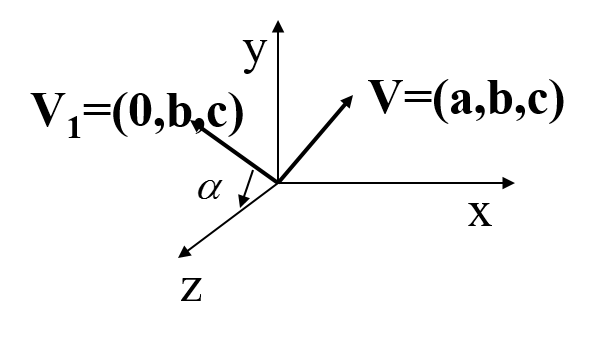
\includegraphics[height=3cm]{geometry/rotate4.png}

$R_x=
\left[
\begin{array}{ c @{\ } c @{\ } c @{\ } c}
    1 & 0                             & 0                            & 0 \\
    0 & \frac{ c }{ \sqrt{b^2+c^2} }  & \frac{ b }{ \sqrt{b^2+c^2} } & 0 \\
    0 & -\frac{ b }{ \sqrt{b^2+c^2} } & \frac{ c }{ \sqrt{b^2+c^2} } & 0 \\
    0 & 0                             & 0                            & 1
\end{array}
\right]
$
\end{frame}

\begin{frame}
\frametitle{第二步}
\pause
以y轴为旋转轴把向量旋入平面yz

V在第一步旋转之后的坐标为$(a,0,\sqrt{b^2+c^2})$,旋转的角度就是现在V与z轴的夹角

\pause
$R_y=
\left[
\begin{array}{ c @{\ } c @{\ } c @{\ } c}
    \frac{ \sqrt{b^2+c^2} }{ \sqrt{a^2+b^2+c^2} } & 0 & \frac{ a }{ \sqrt{a^2+b^2+c^2} }              & 0 \\
    0                                             & 1 & 0                                             & 0 \\
    -\frac{ a }{ \sqrt{a^2+b^2+c^2} }             & 0 & \frac{ \sqrt{b^2+c^2} }{ \sqrt{a^2+b^2+c^2} } & 0 \\
    0                                             & 0 & 0                                             & 1
\end{array}
\right]
$
\end{frame}

\begin{frame}
\frametitle{第三步}
\pause
绕z轴旋转指定的角度$\theta$

$R_z=
\left[
\begin{array}{ c @{\ } c @{\ } c @{\ } c}
    \cos(\theta)  & \sin(\theta) & 0 & 0 \\
    -\sin(\theta) & \cos(\theta) & 0 & 0 \\
    0             & 0            & 1 & 0 \\
    0             & 0            & 0 & 1
\end{array}
\right]
$
\end{frame}

\begin{frame}
\frametitle{第四步}
\pause
把第二步反向还原。即把旋转的角度取相反数，即把sin值取反。

${R'}_y=
\left[
\begin{array}{ c @{\ } c @{\ } c @{\ } c}
    \frac{ \sqrt{b^2+c^2} }{ \sqrt{a^2+b^2+c^2} } & 0 & -\frac{ a }{ \sqrt{a^2+b^2+c^2} }             & 0 \\
    0                                             & 1 & 0                                             & 0 \\
    \frac{ a }{ \sqrt{a^2+b^2+c^2} }              & 0 & \frac{ \sqrt{b^2+c^2} }{ \sqrt{a^2+b^2+c^2} } & 0 \\
    0                                             & 0 & 0                                             & 1
\end{array}
\right]
$
\end{frame}

\begin{frame}
\frametitle{第五步}
\pause
把第一步还原。

${R'}_x=
\left[
\begin{array}{ c @{\ } c @{\ } c @{\ } c}
    1 & 0                            & 0                             & 0 \\
    0 & \frac{ c }{ \sqrt{b^2+c^2} } & -\frac{ b }{ \sqrt{b^2+c^2} } & 0 \\
    0 & \frac{ b }{ \sqrt{b^2+c^2} } & \frac{ c }{ \sqrt{b^2+c^2} }  & 0 \\
    0 & 0                            & 0                             & 1
\end{array}
\right]
$
\end{frame}

\begin{frame}
\frametitle{合并}
\pause
把五个矩阵相乘看起来比较复杂，不过可以强制把向量V模长调整为$\sqrt{a^2+b^2+c^2}=1$

\pause
然后经过一系列复杂的矩阵乘法，可以求出向量旋转的矩阵。

\pause
为了排版方便，令$SIN=\sin(\theta),COS=\cos(\theta)$

$
\left[
\begin{array}{ c @{\ } c @{\ } c @{\ } c}
    a^2+(1-a^2)COS & ab(1-COS)+cSIN & ac(1-COS)-bSIN & 0 \\
    ab(1-COS)-cSIN & b^2(1-COS)+COS & bc(1-COS)+aSIN & 0 \\
    ac(1-COS)+bSIN & bc(1-COS)-aSIN & c^2(1-COS)+COS & 0 \\
    0              & 0              & 0              & 1
\end{array}
\right]
$
\end{frame}

\section{直线}

\subsection{点到直线距离}
\begin{frame}
\pause
三维直线的存储也有两点式和参数式两种。

\pause
求点C到直线AB的距离也类似，$\frac{ \overrightarrow{AB} \times \overrightarrow{AC} } { |AB| }$。

\pause
然后用和二维一样的方法可以求出点到直线的投影。
\end{frame}

\subsection{空中直线距离}
\begin{frame}
\pause
如果两直线有交点，则距离为0。

\pause
如果两直线平行，就相当于是点到直线的距离。

\pause
设两直线的方向向量为$\overrightarrow{a},\overrightarrow{b}$。并且在直线上各任取一点A和B，那么B-A在$\overrightarrow{a} \times \overrightarrow{b}$上的投影的模即为距离。即
\begin{displaymath}
    d=\left| \frac{ (\overrightarrow{a} \times \overrightarrow{b}) \cdot (B-A) }{ |\overrightarrow{a} \times \overrightarrow{b}| } \right|
\end{displaymath}
\end{frame}

\subsection{三维直线求交}
\begin{frame}
\pause
三维直线求交有两种方法。

\pause
第一种是利用与二维直线求交一样的思路，利用叉积算面积并计算。但是这里有一个关键问题：三维叉积求出的是一个向量，向量的模长才是面积，但是求向量的模长需要用到开方操作，这样就丢失了面积的正负。所以我们可以暴力枚举面积正负求出交点再判断是否在直线上。

\pause
第二种是投影法，我们先求出两条直线投影到平面z=0的交点，然后再判断z值是否满足要求。但是这里会遇到特殊情况:$dx=0$或$dy=0$，这时我们需要切换投影面，我们可以把$z=0,y=0,x=0$这三个投影面都尝试一遍，如果都不行则两直线重合或平行，否则就可以找到交点。
\end{frame}

\subsection{异面直线公垂线}
\begin{frame}
\label{hehe}
\pause
求异面直线AB和CD的公垂线PQ。

PQ要同时垂直于AB和CD，则会垂直于AB和CD所在平面，所以就垂直于$\overrightarrow{AB} \times \overrightarrow{CD}$

则$| \overrightarrow{PQ} |=\frac{| \overrightarrow{n} \times \overrightarrow{AC} |}{| \overrightarrow{n} |}$
\end{frame}

\subsection{空中线段距离}
\begin{frame}
\frametitle{求空中线段AB和CD的距离}
\pause
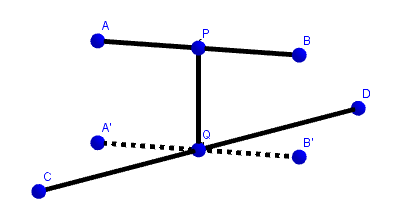
\includegraphics[height=2cm]{geometry/3dline.png}

方法分三步:
\begin{enumerate}
    \item 求出两条线段所在直线的公垂线PQ
    \item 将两个直线投影到与公垂线垂直的平面，计算平面内两条线段的距离dis
    \item $ans=\sqrt{(|PQ|^2+dis^2)}$
\end{enumerate}
令$\overrightarrow{n}=\overrightarrow{AB} \times \overrightarrow{CD}$

公垂线可以用叉积求得。见\textcolor{purple}{\ref{hehe}}

$A'=A+|\overrightarrow{PQ}| \frac{\overrightarrow{n}}{|\overrightarrow{n}|},B'=B+|\overrightarrow{PQ}| \frac{\overrightarrow{n}}{|\overrightarrow{n}|}$
\end{frame}

\section{平面}

\subsection{三维平面表示}
\begin{frame}
\pause
三维平面可以用方程列出一般式，但是一般比较麻烦。

\pause
比较常用的是点法式，用平面上的一个点P和与这个平面垂直的法向量$\overrightarrow{v}$来描述。
\end{frame}

\subsection{点到平面距离}
\begin{frame}
\pause
点A到平面$(P,\overrightarrow{v})$的距离，就是$\overrightarrow{AP}$，在v上的投影长度。
\begin{displaymath}
    \frac{ \overrightarrow{AP} \times \overrightarrow{v} }{ |\overrightarrow{v}| }
\end{displaymath}
\end{frame}

\subsection{点到平面投影}
\begin{frame}
\pause
知道了点到平面的距离，利用法向量就可以求出点到平面的投影。

\pause
有时一些几何对象在同一个平面上，我们希望给予平面上每一个点一个二维坐标，从而把问题转化为一个二维问题解决。

\pause
我们需要在平面上指定一个点O为源点，以及一个向量$\overrightarrow{x}$作为横轴，一个向量$\overrightarrow{y}$作为纵轴，要求$\overrightarrow{x} \bot \overrightarrow{y}$。

对于每一个点A，在当前坐标系下其横坐标为$A-O$在x上的投影长度$\frac{ (A-O) \times \overrightarrow{x} }{ |\overrightarrow{x}| }$，纵坐标亦然。

\pause
为了方便，我们可以把$| \overrightarrow{x} |$和$| \overrightarrow{y} |$缩放为1。

若已知平面上一点以此坐标系投影的坐标为$(a,b)$，则还原到三维坐标为$O+a\overrightarrow{x}+b\overrightarrow{y}$
\end{frame}

\subsection{直线和面交点}
\begin{frame}
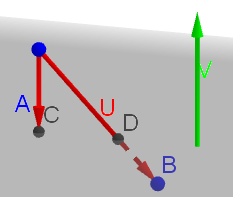
\includegraphics[height=3cm]{geometry/3dgraph.png}

求直线AB和平面$(C,\overrightarrow{v})$的交点。

首先求出A到平面C的垂直向量$\overrightarrow{AC}$

如果$\overrightarrow{AB} \perp \overrightarrow{AC}$则线面平行，无解。

否则我们需要找到的点D满足$\overrightarrow{AD}$在$\overrightarrow{AC}$上的投影恰好为$\overrightarrow{AC}$。即$\overrightarrow{AD} \times \overrightarrow{AC}=|AC|^2$

同时$\overrightarrow{AD}:\overrightarrow{AB}=| \overrightarrow{AD} \times \overrightarrow{AC} |:|\overrightarrow{AB} \times \overrightarrow{AC} |$

所以$\overrightarrow{AD}=\overrightarrow{AB}
\frac{ | \overrightarrow{AD} \times \overrightarrow{AC} |}{|\overrightarrow{AB} \times \overrightarrow{AC} |}
=\overrightarrow{AB} \frac{|AC|^2}{| \overrightarrow{AB} \times \overrightarrow{AC} |}$

\end{frame}

\subsection{面和面的交线}
\begin{frame}
设两平面的法向量为$h_1,h_2$。

若它们平行，则两平面平行或重合。

否则，交线的方向向量与$h_1,h_2$垂直，即为$h_1 \times h_2$，那么就只需求出交线上的一点即可。

可以随机生成一条在第一平面内，但不与第二平面平行的直线，求它与第二平面的交点。
\end{frame}

\subsection{二面角}
\begin{frame}
\pause
就是两个平面法向量的夹角。
\end{frame}

\section{球}
\subsection{球与直线的交点}
\begin{frame}
\pause
首先求球心到直线的距离h和垂足。

\pause
若$h>r$则无解。

\pause
两个交点到垂足的距离为$\sqrt{r^2-h^2}$，缩放直线向量求得即可。
\end{frame}

\subsection{球与平面或球的交圆}
\begin{frame}
\pause
先求交圆的圆心，再求出半径。因为是三维空间，所以还要表面圆所在的平面。
\end{frame}

\section{三维凸包}

\subsection{定义}
\begin{frame}
\pause
同二维凸包一样定义：如果点集中存在点A,B，则线段AB上的所有点都必须在凸包内

\pause
不过还要加上一条：凸包的每一个面都满足，所有点只会分布在面的一侧。

\pause
在满足这两个条件的情况下，取体积最小的多面体。

\pause
结论：三维凸包的边数是线性的

\pause
证明：我们可以把三维凸包的表面展开成一个平面图。由欧拉公式，F(面数)+V(点数)-E(边数)=2

一条边恰归属于两个面，一个面有$\ge 3$条边，$2E \ge 3F$。

可得$E \le 3V-6,F \le 2V-4$
\end{frame}

\subsection{构造}

\begin{frame}
\frametitle{方法一}
\framesubtitle{暴力法}
\pause
可以很自然地想到一种暴力：

\pause
$O(n^3)$枚举每一个面，然后$O(n)$check一下每一个点是否都在面内。
\end{frame}

\begin{frame}
\frametitle{方法二}
\framesubtitle{增量法}
\pause
先取出点集中的4个点，这4个点组成的四面体为初始凸包。(要求这4个点构成的凸包体积不为0)

然后添加其他各点。如果这个点在已知凸包内部，则直接跳过。否则，找出可视部分与不可视部分的分界线，删去所有的可视面，然后将所有分界线上的边与该点构成的面作为新凸包的面。

\begin{multicols}{2}
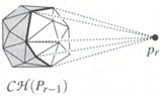
\includegraphics[height=2cm]{geometry/3dtubao.png}

黑色的边被称为地平线。地平线的两端，一定是一个可见面一个不可见面。

然后删除可见面，用新点连接地平线的每一条边。
\end{multicols}

\pause
要注意的是一个面上的点的顺序，两个不同的顺序代表的是两个不同的半空间。
\pause
复杂度$O(n^2)$。同时这个方法是在线的。
\end{frame}

\begin{frame}
\frametitle{方法三}
\framesubtitle{卷包裹法}
\pause
卷包裹法就是一张纸紧贴着凸包的一条边AB沿AB的右手边收拢，直到遇到顶点C为止

那么ABC是凸包上的一个面

递归：沿$AC$和$CB$方向搜索

\pause
初始时找到一条一定在凸包中的边$AB$，然后调用函数$wrap(\overrightarrow{AB})$

\pause
复杂度$O(nh)$
\end{frame}

\begin{frame}
\frametitle{方法四}
\framesubtitle{随机增量法}
\pause
方法二的增量复杂度瓶颈在于每次都要扫描所有凸包上的边来找到可见面与不可见面的边界。

考虑增量算法的一个改进，寻找地平线时不枚举所有面，而是利用之前的信息

\pause
定义二分图$C=(P,F,E)$，如果一个点P看得到一个面F，在他们之间连边，得到的二分图称为冲突图(conflict graph)

冲突图的两部分别是未处理的点和已存在的面
\end{frame}

\begin{frame}
\frametitle{方法四}
\framesubtitle{随机增量法}
\pause
\begin{multicols}{2}
查询可见面:

直接从冲突图里面读取

设置点为已处理，删除平面:

直接对二分图进行操作

加入新面:

枚举每个点，判断可见性

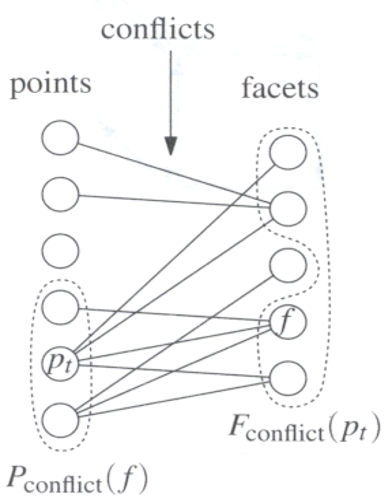
\includegraphics[height=5cm,width=4cm]{geometry/3dtubao2.png}
\end{multicols}

但是加入新面时还是要扫一遍所有的点，复杂度仍然是平方。
\end{frame}

\begin{frame}
\frametitle{方法四}
\framesubtitle{随机增量法}
\pause
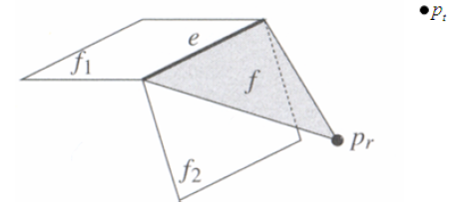
\includegraphics[height=3cm]{geometry/3dtubao3.png}

新的面一定连接当前处理点Pr和一条地平线e

假设e原先连接两个面f1,f2（恰好有一个面将被剔除）

证明：点Pt若能看见f，必定能看见f1或f2

在加入facet时只需要考虑能见到f1/f2的点

\pause
据说复杂度是$nlogn$的，但是并不会证明。不过实际复杂度确实非常优秀。
\end{frame}

\begin{frame}
\frametitle{方法五}
\framesubtitle{分治法}
\pause
和2维一样的思路，分块构造凸包，然后进行合并。 \newline \newline

\pause
鉴于三维凸包的合并非常复杂，并且很容易把复杂度写挂，所以仅供了解。
\end{frame}

\begin{frame}
\frametitle{方法六}
\framesubtitle{QuickHull}
\pause
把二维的情况稍稍拓展就可以做三维了。

调用函数$Quickhull(P_0,P_1,P_2)$

找到离平面$(P_0,P_1,P_2)$最远的点K

递归:

$Quickhull(K,P_0,P_1)$

$Quickhull(K,P_1,P_2)$

$Quickhull(K,P_2,P_0)$ \newline \newline

\pause
同样，Quickhull算法被经常运用在三维乘积问题中。(如三维最小乘积生成树)
\end{frame}

\subsection{三维凸包的体积、重心}
\begin{frame}
\frametitle{重心}
\pause
几何定义：顶点和对面重心的连线交点为重心。
$G=\frac{A+B+C+D}{4}$

\pause
可以推广到N维单纯形上

\pause
多面体重心：

以原点进行三角剖分

\begin{displaymath}
G=\frac{\sum V_iG_i}{\sum V_i}
\end{displaymath}

假设各个面是$i \rightarrow j \rightarrow k$

\begin{displaymath}
G_i=\frac{P_i+P_j+P_k}{4},V_i=\frac{(P_i \times P_j) \cdot P_k}{6}
\end{displaymath}

\begin{displaymath}
G= \sum_i \frac{(P_i+P_j+P_k)*((P_i \times P_j) \cdot P_k)}{24V}
\end{displaymath}
\end{frame}

\subsection{三维半空间交}
\begin{frame}
\textcolor{red}{\huge{我不会。。。QAQ}}
\end{frame}
